\chapter{Experiments and Results}\label{Chapter5:Experiments and Results}
We have experimented with a large number of configurations using the ChampSim simulator. In the following, we will discuss the details of the results. The highlights include performance improvement on top of SPP in single-core high bandwidth configuration and reduction in prefetch bandwidth at the DRAM and the LLC while maintaining SPP performance. In multiprogrammed workloads, our proposal delivers performance close to SPP while consuming less bandwidth. We will also discuss experiments with varying prefetch depths and threshold values offering us more insights into the behaviour of SPP and the proposed improvements. 

The following prefetcher configurations are evaluated. These prefetcher configurations are used only at L2C and there is no prefetcher at L1C and LLC. These are evaluated for single-core as well as quad-core environments. For the quad-core environments, we will report results for homogeneous~(rate mode) and heterogeneous multiprogrammed workloads.
\begin{itemize}
    \item{Baseline SPP}
    \item{SPP working with only critical load addresses}
    \item{SPP with changed threshold}
    \item{Enhanced SPP lookahead mechanism with less bandwidth proposal}
    \item{Enhanced SPP lookahead mechanism with higher bandwidth proposal~(depth version)}
\end{itemize}
To evaluate the results, we use the following metrics.
\begin{itemize}
    \item{Geometric mean of IPCs over all the traces}
    \item{Average L2C, LLC,  and DRAM Bandwidths over all the traces}
    \item{Average number of addresses input to the prefetcher over all the traces}
    \item{Average accuracy of the prefetches at the L2C and LLC over all the traces.}
    \item{Comparison of the depth-critical Workloads individually} 
\end{itemize}
Depth-critical workloads are those which experience significant increase in IPC when depth or total number of prefetches increases. In the following results, cache and DRAM bandwidth means the total number of prefetch requests to the cache and DRAM, respectively. For example, DRAM bandwidth means total number of prefetch requests from LLC to DRAM.

For high-bandwidth configurations, we set the pattern table way~(PT\_WAY) to 2 instead of 4 because in this case, the prefetcher explores higher depths and we get fine-grain control over the total number of prefetches generated by having a lower value of PT\_WAY.
In the simulations of  multi-programmed workloads, we set the threshold for dynamic ROB head stall to one-seventh of the largest delay from the last interval. For single-core simulations, this is set to one-quarter of the highest delay. This is done because of increased bandwidth consumption and cache pollution in multi-core configurations. 

\section{Single Core Results}
\begin{figure}[H]
{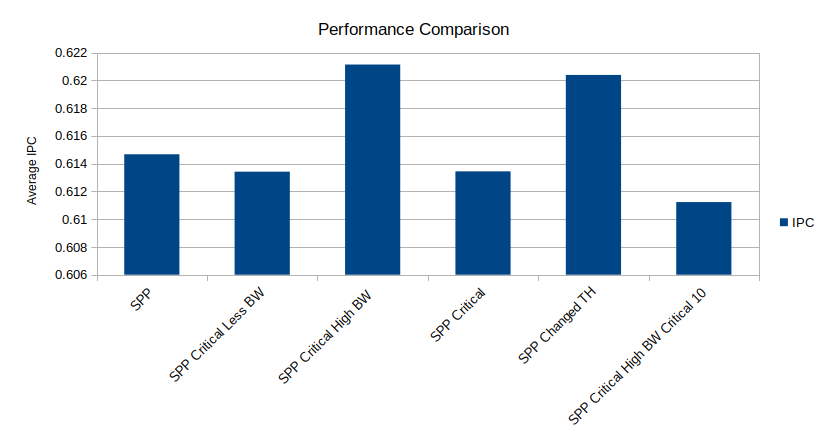
\includegraphics[scale=0.5]{images/IPC_single.png}}
\caption{Performance comparison for single-core configuration}
\label{fig:single-core-perf}
\end{figure}

Figure~\ref{fig:single-core-perf} shows the single-core performance for different configurations, while Figures~\ref{fig:l2c-prefetch-count}, \ref{fig:llc-prefetch-count}, and~\ref{fig:dram-prefetch-count} respectively show the number of prefetch lookups at the L2C, LLC, and DRAM.
For single core, our less bandwidth proposal~(SPP Critical Less BW) performs similar to SPP with 4-5\% less LLC and DRAM bandwidth consumption. If we pass only critical load addresses to the SPP~(SPP Critical), we get approximately same performance but with less L2C and LLC bandwidth consumption.
\begin{figure}[H]
{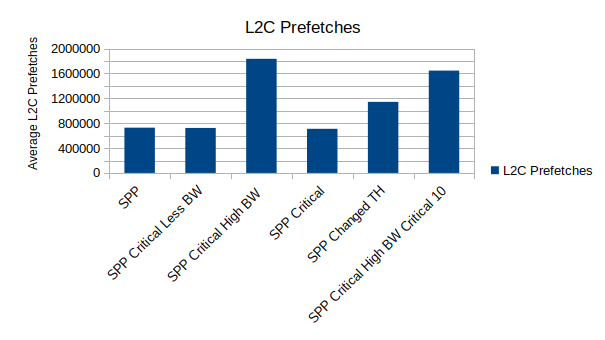
\includegraphics[scale=0.7]{images/single_core_L2C_BW.png}}
\caption{Number of prefetch lookups at L2C for single-core configuration}
\label{fig:l2c-prefetch-count}
\end{figure}

In the high bandwidth proposal~(SPP Critical High BW), we prefetch using higher depths for every source address. Compared to SPP, we get about 1\% improvement in IPC, but require almost 2.5$\times$ more L2C bandwidth and 36\% more LLC bandwidth. If we compare it with a configuration where for every address passed to SPP, it prefetches till depth ten~(SPP Critical High BW Critical 10) then we get only 0.2\% performance improvement while consuming 11\% more L2C bandwidth but with 41\% and 40\% less LLC and DRAM bandwidth respectively. In some cses, our high bandwidth prefetching proposal goes till depth 12 and because of this, we consume more L2C bandwidth in these cases. However, overall, our high bandwidth proposal is able to convert this bandwidth consumption into reasonable performance improvement~(average 1\% IPC improvement is significant considering the large number of traces).
\begin{figure}[H]
{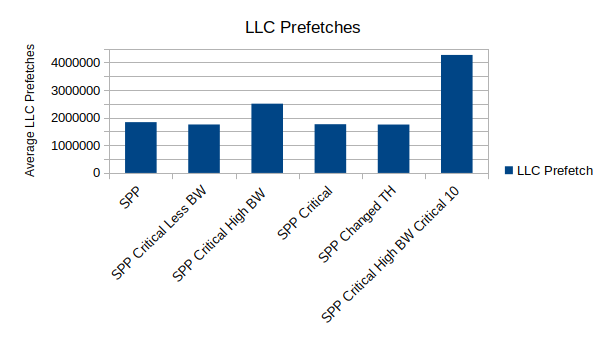
\includegraphics[scale=0.7]{images/single_core_LLC_Bandwidth.png}}
\caption{Number of prefetch lookups at LLC for single-core configuration}
\label{fig:llc-prefetch-count}
\end{figure}

We also experimented by varying the PF\_Threshold and Fill\_Threshold in SPP. These results are shown in the bar marked ``SPP Changed TH''.
If we increase PF\_Threshold by 5 and decrease Fill\_Threshold by 5 in SPP, it results in almost 1\% performance improvement while requiring 57\% more L2C prefetch lookups and about 5\% less LLC and 6\% less DRAM prefetch lookups. This allows more prefetches at L2C, but prefetched blocks with lower confidence are filled in the LLC only. However, it still require all the load addresses to be passed to the prefetcher as in SPP, thereby increasing the prefetcher activity and energy expense quite significantly.
\begin{figure}[H]
{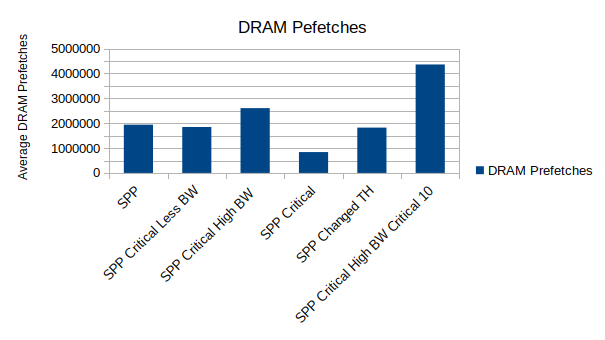
\includegraphics[scale=0.7]{images/DRAM BW comparison single core.png}}
\caption{DRAM prefetch request count for single core configuration}
\label{fig:dram-prefetch-count}
\end{figure}
\begin{figure}[H]
{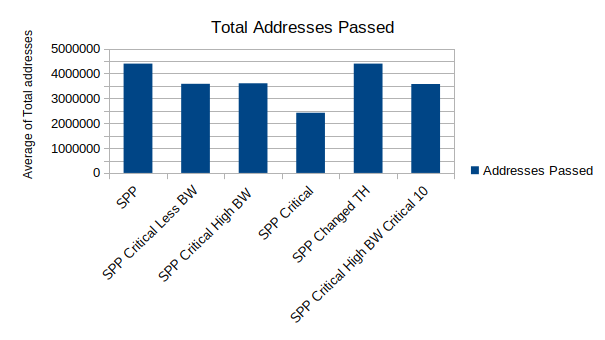
\includegraphics[scale=0.7]{images/Total Addresses single.png}}
\caption{Number of load addresses passed to SPP for single core configuration}
\label{fig:address-passed}
\end{figure}

To understand the savings in the activity of the prefetcher due to criticality-based filtering, Figure~\ref{fig:address-passed} shows the number of load addresses passed to the prefether for various configurations. 
Because SPP uses more sophisticated lookahead mechanism, when we pass only the critical load addresses to it~(SPP Critical), it results in 56\%  less DRAM Bandwidth consumption and 45\% less total addresses passed to the prefetcher with slightly lower IPC compared to the baseline SPP. The baseline SPP processes 22\% more input addresses compared to the less bandwidth and high bandwidth proposals.

Figure~\ref{fig:accuracy-single-core} shows the accuracy of the prefetches as seen by the L2C and LLC.
The prefetch accuracy at L2C is close to 96\% for the less bandwidth proposal and 85\% for the high bandwidth proposal. This is an expected result because the less bandwidth proposal is more selective about prefetching.
\begin{figure}[H]
{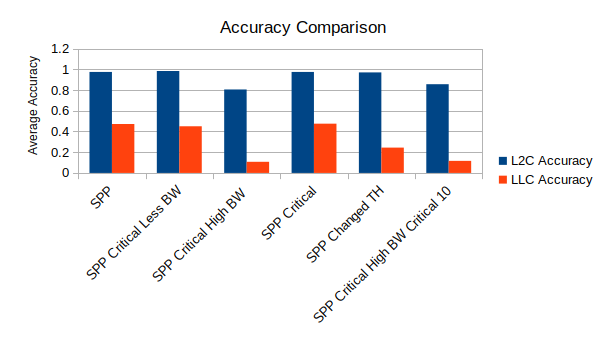
\includegraphics[scale=0.7]{images/Accuracy Comparison_single.png}}
\caption{Accuracy of prefetches at L2C and LLC for single core configuration}
\label{fig:accuracy-single-core}
\end{figure}

The prefetch accuracy at LLC is around 45\% for the less bandwidth proposal and around 10\% for the high bandwidth proposal. The LLC accuracy is low because most of the prefetched blocks get inserted in both L2C and LLC and most of the demand hits are served by L2C obviating the need to look up the LLC. Additionally, the high bandwidth proposal is likely to pollute the caches with a large number of inaccurate prefetches.
\begin{figure}[H]
{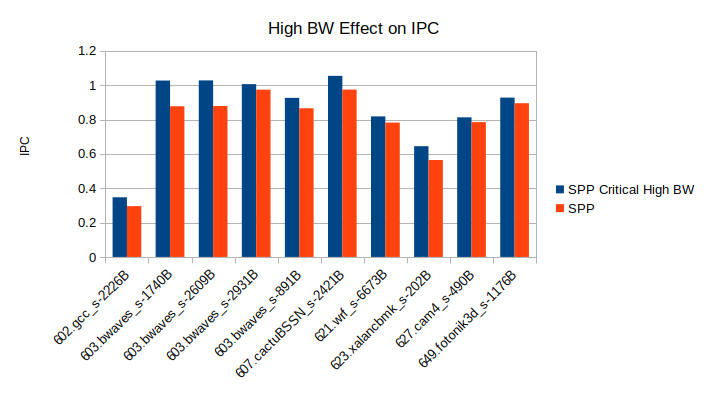
\includegraphics[scale=0.6]{images/Depth_critical workloads.png}}
\caption{Analysis of high bandwidth proposal's effect on IPC for single core configuration}
\label{fig:high-bw-analysis}
\end{figure}

Since our high bandwidth critical load proposal improved the average performance quite reasonably, we examine the individual workloads
which enjoy significant performance improvement with this proposal in Figure~\ref{fig:high-bw-analysis}. These workloads continue to inject more useful prefetches at higher depths. Performance can be further increased if we use some kind of filtering of prefetches that can reduce the pollution, keep the good prefetches, and increase the prefetch accuracy.

\section{High Bandwidth Proposal with Different Depths}

To see the behaviour of SPP with critical addresses at high bandwidth and to find out the optimal depth, we conducted experiments with different depth values. In these experiments,
we predict the fill level of the prefetches and no address is dropped; all of them insert prefetched blocks at L2C or LLC depending on the fill level.
\begin{figure}[H]
{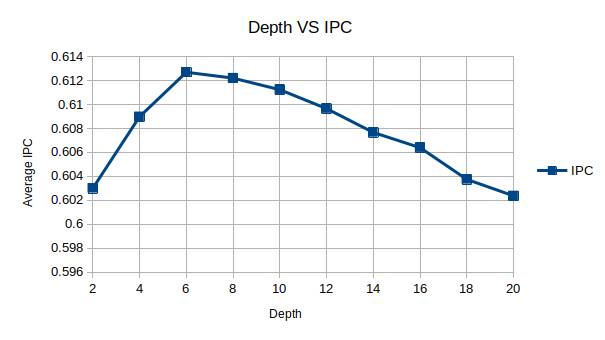
\includegraphics[scale=0.7]{images/IPC vs Depth.png}}
\caption{Depth vs. IPC for single core configuration}
\label{fig:depth-ipc}
\end{figure}

Figure~\ref{fig:depth-ipc} shows the variation in IPC with depth.
We can see a skewed bell curve with its peak at depth six. We see steep increases in IPC from 2 to 4 depth and 4 to 6 depth. This may be due to the fact that there are many workloads which take advantage of increased prefetch depths. After that the average IPC starts decreasing, although certain individual workloads continue to enjoy improved performance which is why the decline in average IPC is rather slow.
\begin{figure}[H]
{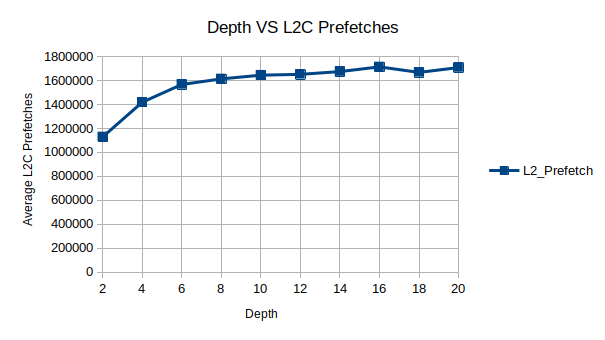
\includegraphics[scale=0.7]{images/L2 Prefetches vs Depth.png}}
\caption{Depth vs. L2C prefetch count for single core configuration}
\label{fig:depth-l2cpref}
\end{figure}

Figure~\ref{fig:depth-l2cpref} shows the number of L2C prefetched block insertions as a function of depth.
L2C prefetch count increases as we increase depth and after a point it becomes nearly a constant. It is because the parameters we use like accuracy of prefetches at any level start decreasing and once they go below a threshold value, the prefetches are blocked from inserting into the L2C.
\begin{figure}[H]
{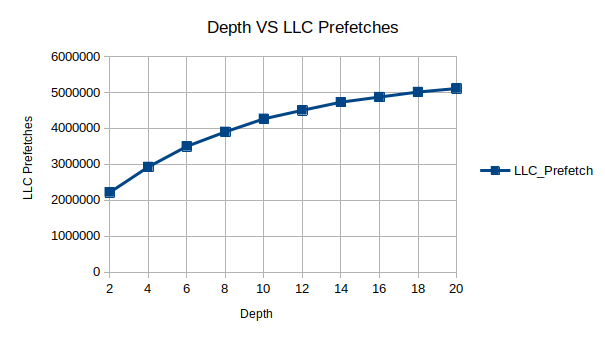
\includegraphics[scale=0.7]{images/LLC Prefetches vs Depth.png}}
\caption{Depth vs. LLC prefetch count for single core configuration}
\label{fig:depth-llcpref}
\end{figure}
\begin{figure}[H]
{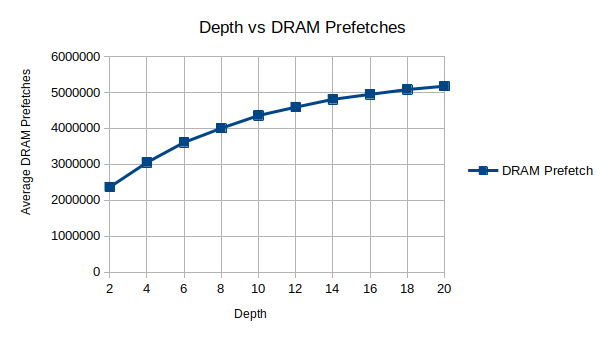
\includegraphics[scale=0.7]{images/Depth VS DRAM BW.png}}
\caption{Depth vs. DRAM prefetch count for single core configuration}
\label{fig:depth-drampref}
\end{figure}

Figures~\ref{fig:depth-llcpref} and~\ref{fig:depth-drampref} respectively show the LLC and DRAM prefetch counts as a function of prefetch depth. These functions have the shape of a quadratic.
Because parameters at LLC have lower threshold values than at L2C, a much higher depth is needed for the prefetch count to start declining.
These thresholds decide whether to insert a prefetched block at a cache level or not.
\begin{figure}[H]
{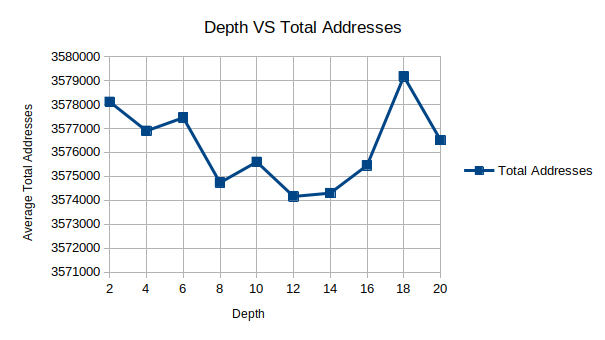
\includegraphics[scale=0.7]{images/Depth vs Critical Addresses.png}}
\caption{Depth vs. number of addresses input to the prefetcher for single core configuration}
\label{fig:depth-address}
\end{figure}

Figure~\ref{fig:depth-address} shows the number of addresses input to the prefetcher as a function of depth.
We can see some variation in total number of addresses passed to the prefetcher (only critical addresses are passed). The variation arises primarily due to cache  pollutions, but there are other factors also. The more misses a workload generates, it will make other IPs wait at the ROB head leading to generation of more critical loads and more prefetches as the depth increases.

\section{Quad-core Homogeneous Results}

Each core has private L2C. The LLC is shared among the cores. The shared LLC can become congested for higher bandwith demands. In the following, we discuss the results for homogeneous multi-programmed workloads where all four cores run the same Workload.

Figure~\ref{fig:multicore-ipc} shows the average IPC of different configurations, while Figures~\ref{fig:multicore-l2cpref}, \ref{fig:multicore-llcpref}, and~\ref{fig:multicore-drampref} quantify the number of prefetches respectively at L2C, LLC, and DRAM.
We can see that our high bandwidth proposal generates lots of L2C prefetches (2.5$\times$ more than SPP), LLC prefetches (36\% more than SPP), and DRAM prefetches (31\% more than SPP). Therefore, the homogeneous multi-core workloads were not able to take advantage of aggressive prefetching. The performance of the high bandwidth proposal is 2.6\% lower than SPP.
\begin{figure}[H]
{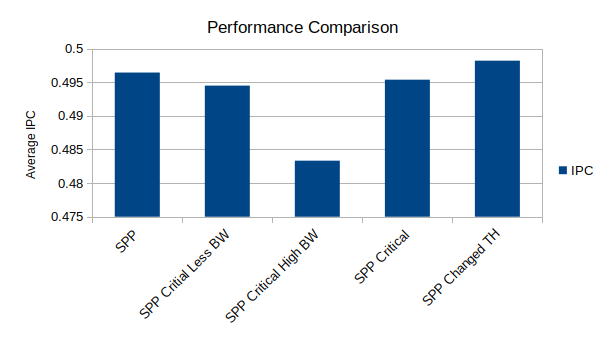
\includegraphics[scale=0.7]{images/IPC_Homo.png}}
\caption{Performance comparison for quad-core homogeneous workloads}
\label{fig:multicore-ipc}
\end{figure}
\begin{figure}[H]
{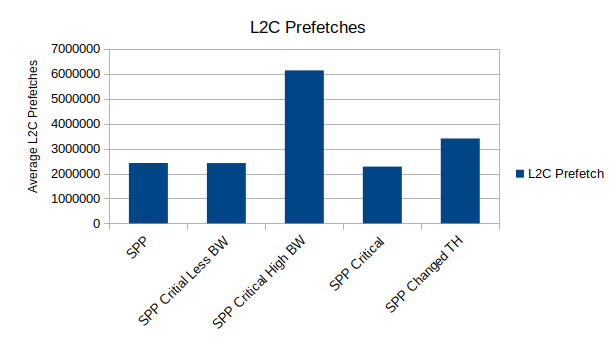
\includegraphics[scale=0.7]{images/L2C_Homo.png}}
\caption{Number of L2C prefetches for quad-core homogeneous workloads}
\label{fig:multicore-l2cpref}
\end{figure}

The low bandwidth proposal results in approximately the same L2C prefetches and approximately 5\% less LLC and 5.6\% less DRAM prefetches. Also, its performance is only 0.3\% lower than SPP.
\begin{figure}[H]
{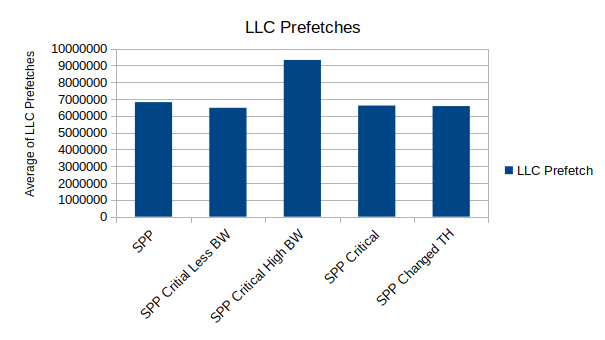
\includegraphics[scale=0.7]{images/LLC_Homo.png}}
\caption{Number of LLC prefetches for quad-core homogeneous workloads}
\label{fig:multicore-llcpref}
\end{figure}
\begin{figure}[H]
{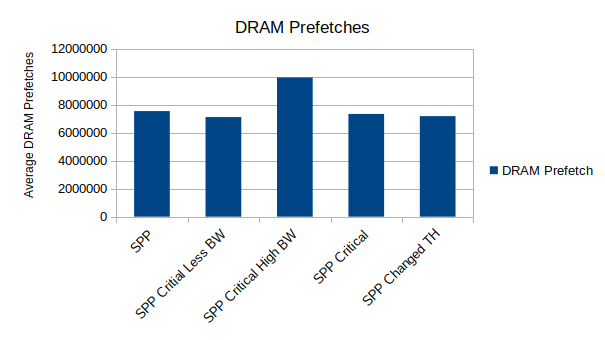
\includegraphics[scale=0.7]{images/DRAM BW Homo.png}}
\caption{Number of DRAM prefetches for quad-core homogeneous workloads}
\label{fig:multicore-drampref}
\end{figure}

SPP with only critical addresses behaves almost similarly as SPP with 0.2\% lower performance and 6\% less L2C and 3\% less LLC and DRAM prefetches. 
\begin{figure}[H]
{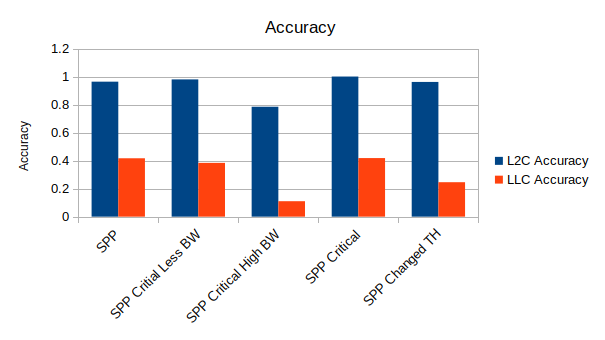
\includegraphics[scale=0.7]{images/Accuracy_homo.png}}
\caption{Accuracy comparison for quad-core homogeneous workloads}
\label{fig:multicore-accuracy}
\end{figure}

Changing PF\_THRESHOLD and FILL\_THRESHOLD gives us 0.3\% performance improvement over SPP with 40\% more L2C prefetches, 3.4\% less LLC and 5\% less DRAM prefetches. This is because even though we allow more prefetches in L2C and less in LLC, the internal SPP lookahead mechanism throttles the prefetch lookahead more efficiently. It is also because SPP has more addresses and can learn more efficiently.     
The number of addresses passed to the prefetcher is 20\% less in SPP with critical addresses than in SPP~(Figure~\ref{fig:multicore-addr}). Also, due to high pollution in the high bandwidth proposal, it has lower L2C and LLC prefetetch accuracy~(Figure~\ref{fig:multicore-accuracy}).
\begin{figure}[H]
{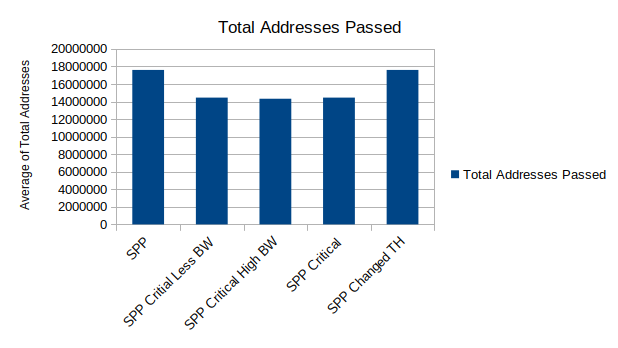
\includegraphics[scale=0.7]{images/Total _addresses_homo.png}}
\caption{Number of addresses input to the prefetcher for quad-core homogeneous workloads}
\label{fig:multicore-addr}
\end{figure}

\section{Quad-Core Heterogeneous Workloads}

We combine four random single-core workloads to build 95 different heterogeneous quad-core workloads. Every single-core workload occurs four times in the combinations ensuring unbiased representation of all the single-core workloads. 

Figure~\ref{fig:hetero-perf} shows the performance, while Figures~\ref{fig:hetero-l2cpref}, \ref{fig:hetero-llcpref}, and~\ref{fig:hetero-drampref} quantify the number of prefetches respectively at L2C, LLC, and DRAM.
Performance for the high bandwidth proposal is approximately 1.6\% lower than SPP. It consumes almost 3$\times$ more L2C bandwidth than SPP. However, it consumes only 10\% more LLC and DRAM bandwidth than SPP. Unlike in homogeneous workloads, in heterogeneous case the cores compete for LLC for different data in all configurations. The
less bandwidth proposal consumes 1.4\% less L2C bandwidth, 10\% less LLC bandwidth and DRAM prefetches, and results in 1.1\% lower performance than SPP.
We have also experiemented by changing the pattern table ways from 4 to 2 for other configurations apart from the high bandwidth and it resulted in less performance reduction.
But we have presented the result for PT\_WAY of 2 for having uniform parameter settings across all results.
By changing the threshold values we get 0.5\% more performance with 46\% more L2C bandwidth, 1.8\%  less LLC and 2.4\% less DRAM prefetches than SPP.
\begin{figure}[H]
{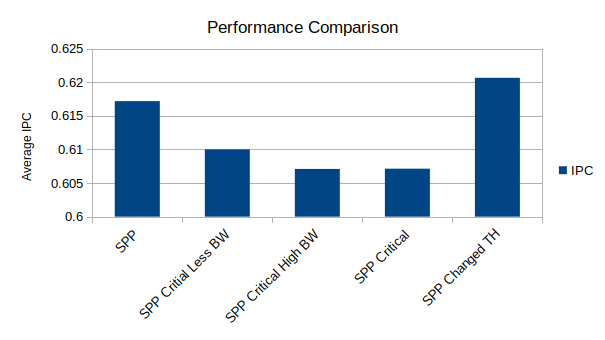
\includegraphics[scale=0.7]{images/IPC_Hetro.png}}
\caption{Performance comparison for quad-core hetroogeneous workloads}
\label{fig:hetero-perf}
\end{figure}

The LLC and DRAM prefetch counts for SPP are very high for heterogeneous workloads, Whereas the less bandwidth proposal and SPP Critical configuration have approximatey 10\% less LLC and DRAM prefetches. 
\begin{figure}[H]
{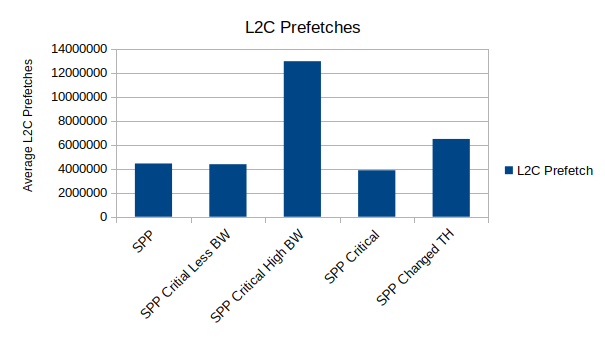
\includegraphics[scale=0.7]{images/L2C_Hetro.png}}
\caption{L2C prefetch count comparison for quad-core heterogeneous workloads}
\label{fig:hetero-l2cpref}
\end{figure}
\begin{figure}[H]
{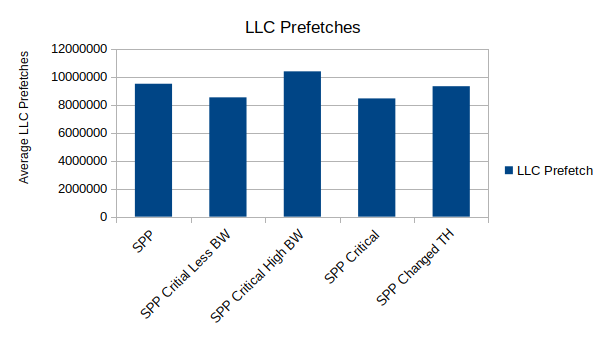
\includegraphics[scale=0.7]{images/LLC_Hetro.png}}
\caption{LLC prefetch count comparison for quad-core heterogeneous workloads}
\label{fig:hetero-llcpref}
\end{figure}
\begin{figure}[H]
{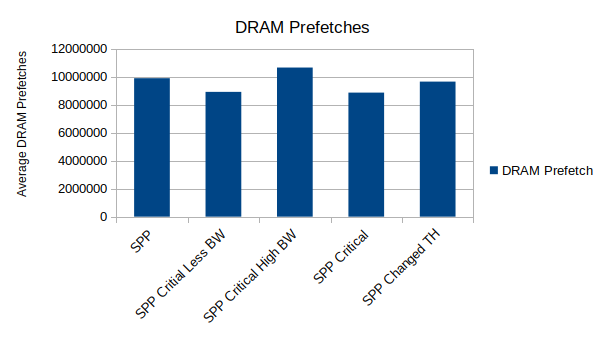
\includegraphics[scale=0.7]{images/DRAM BW Hetro.png}}
\caption{DRAM prefetch count comparison for quad-core heterogeneous workloads}
\label{fig:hetero-drampref}
\end{figure}
\begin{figure}[H]
{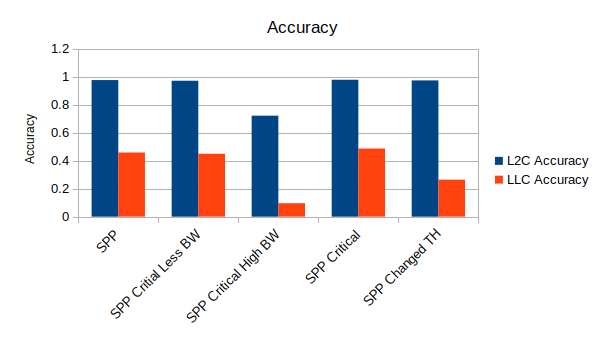
\includegraphics[scale=0.7]{images/Accuracy_hetro.png}}
\caption{Accuracy comparison for quad-core heterogeneous workloads}
\label{fig:hetero-accuracy}
\end{figure}
\begin{figure}[H]
{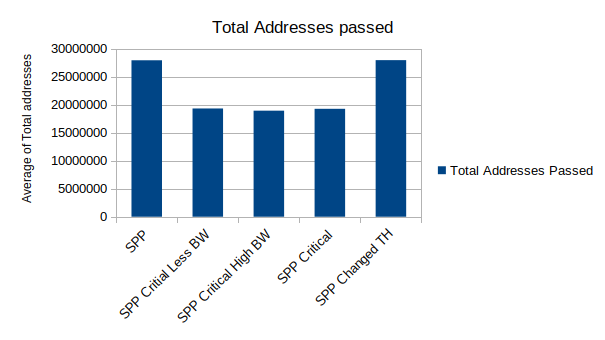
\includegraphics[scale=0.7]{images/Total Addresses_hetro.png}}
\caption{Number of addresses input to the prefetcher for quad-core heterogeneous workloads}
\label{fig:hetero-addr}
\end{figure}

Prefetch accuracy~(Figure~\ref{fig:hetero-accuracy}) and the number of addresses input to the prefetcher~(Figure~\ref{fig:hetero-addr}) also behave similarly as in the homogeneous workloads with the high bandwidth proposal having lower accuracy.
The major difference between homogeneous and heterogeneous workloads is that SPP generates lots of LLC and DRAM prefertches, while our less bandwidth configuration is able to handle it in the heterogeneous case.